\chapter{Groupes caractéristiques et familles}\label{ch:g11:functional-groups}

Ouvrez une bouteille de vinaigre, un flacon de dissolvant pour vernis,
un sachet de bonbons acidulés à la poire, et passez devant l'étal d'un
poissonnier~: quatre odeurs, piquante, sucrée de \omterm{def:g6:solutions-and-solubility:solute}{solvant}, fruitée et
poissonneuse, et quatre sortes de \omterm{def:g7:atoms-and-molecules:molecule}{molécules} différentes. Chacune doit son
odeur, et l'essentiel de sa chimie, non pas à son squelette carboné mais
à un petit groupe d'\omterm{def:g7:atoms-and-molecules:atom}{atomes} fixé sur lui~: de l'oxygène et de l'hydrogène
à un endroit, un \omterm{def:g7:atoms-and-molecules:atom}{atome} d'azote à un autre. Les chimistes classent les
\omterm{def:g11:organic-skeletons:organic}{composés organiques} selon ces groupes.

\begin{recall}
Les \omterm{def:g11:organic-skeletons:formulas}{formules topologiques}, les noms des \omterm{def:g11:organic-skeletons:alkane}{alcanes} et des \omterm{def:g11:organic-skeletons:alkane}{groupes alkyle},
les \omterm{def:g11:organic-skeletons:isomer}{isomères} (\cref{ch:g11:organic-skeletons}). Les \omterm{def:g11:polarity-and-cohesion:polar-bond}{liaisons polarisées}
et les \omterm{def:g11:polarity-and-cohesion:hydrogen-bond}{liaisons hydrogène} (\cref{ch:g11:polarity-and-cohesion}).
\end{recall}

\begin{omfigure}
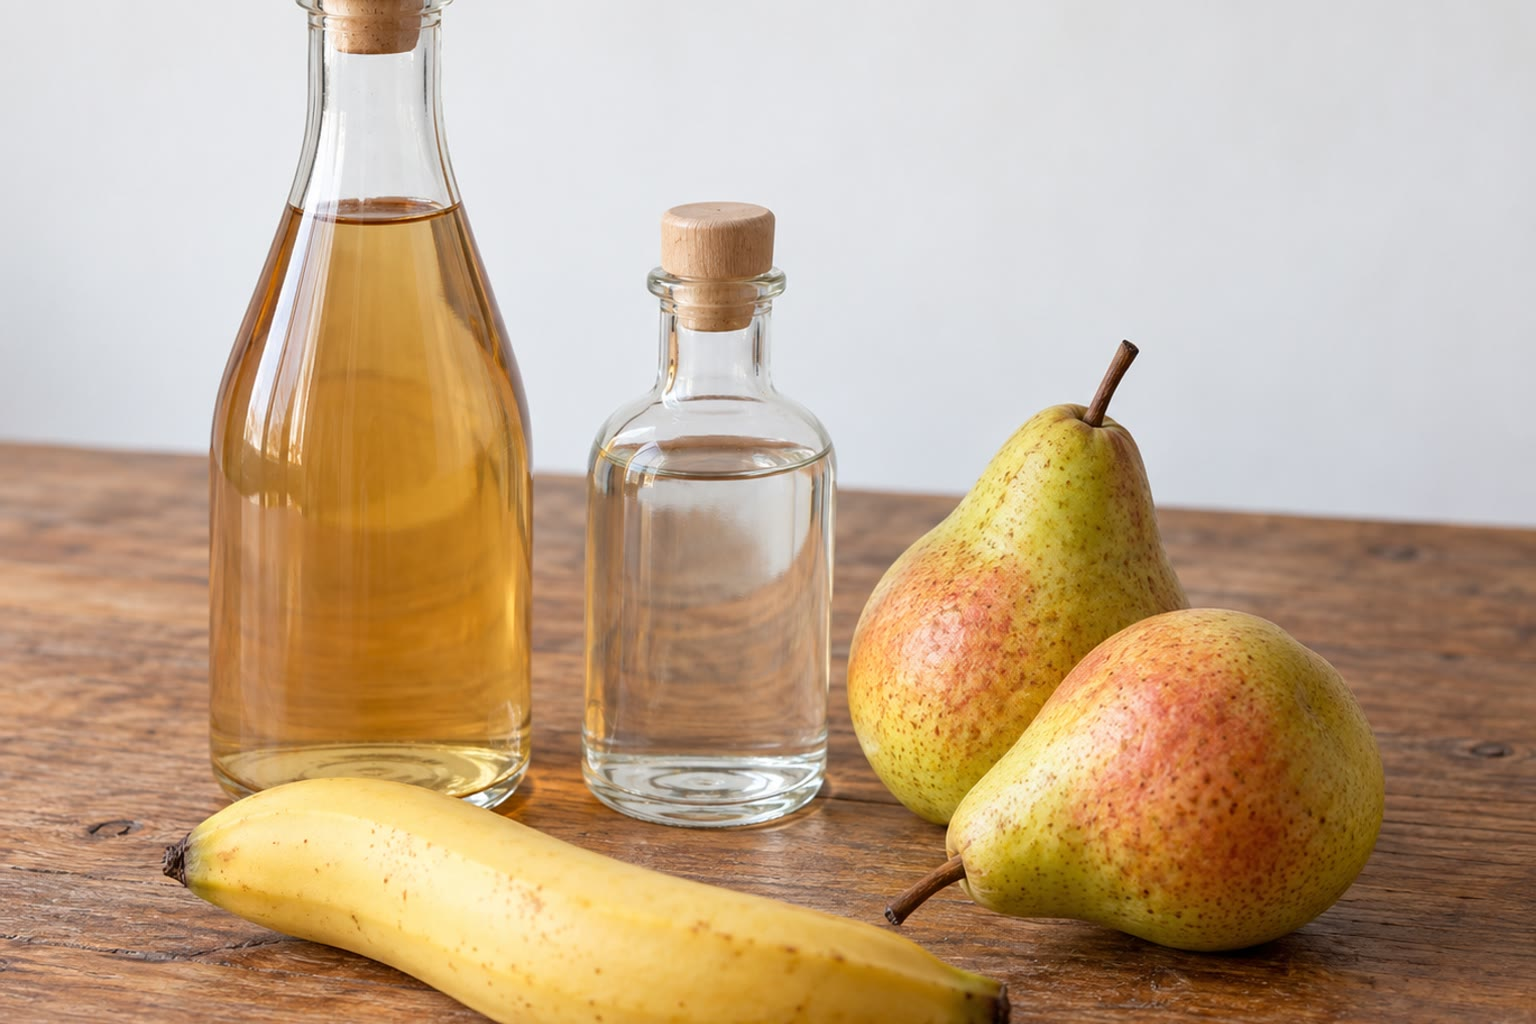
\includegraphics[width=0.5\linewidth]{images/book1/ai/g11-still-life-esters.jpg}

{\small Du vinaigre, un \omterm{def:g6:solutions-and-solubility:solute}{solvant}, des fruits~: chaque odeur vient d'un
groupe d'\omterm{def:g7:atoms-and-molecules:atom}{atomes} différent porté par un squelette carboné.}
\end{omfigure}

\section{Les groupes caractéristiques}

\begin{definition}[Groupe caractéristique]\label{def:g11:functional-groups:functional-group}
Un \emph{groupe caractéristique}\index{groupe caracteristique@groupe caractéristique} est un
groupe d'\omterm{def:g7:atoms-and-molecules:atom}{atomes}, autre que les \omterm{def:g7:atoms-and-molecules:atom}{atomes} de carbone et d'hydrogène du
squelette reliés uniquement par des liaisons simples, qui donne à une
\omterm{def:g7:atoms-and-molecules:molecule}{molécule} ses réactions caractéristiques. Les composés qui ont en commun
un groupe caractéristique forment une famille fonctionnelle.
\end{definition}

\begin{omfigure}
\renewcommand{\arraystretch}{1.35}
\footnotesize
\begin{tabular}{@{}l@{\enspace}l@{\enspace}l@{\enspace}l@{\enspace}l@{}}
\hline
groupe & formule & famille & terminaison & exemple \\
\hline
hydroxyle & \ce{-OH} & \omterm{def:g11:functional-groups:alcohol}{alcool} & \emph{-ol} & éthanol, \ce{CH3-CH2-OH} \\
carbonyle (bout) & \ce{-CHO} & \omterm{def:g11:functional-groups:carbonyl}{aldéhyde} & \emph{-al} & éthanal, \ce{CH3-CHO} \\
carbonyle (milieu) & \ce{C-CO-C} & \omterm{def:g11:functional-groups:carbonyl}{cétone} & \emph{-one} & propanone, \ce{CH3-CO-CH3} \\
carboxyle & \ce{-COOH} & \omterm{def:g11:functional-groups:carboxylic-acid}{acide carboxylique} & \emph{acide \ldots-oïque} & acide éthanoïque, \ce{CH3-COOH} \\
\omterm{def:g11:functional-groups:carboxylic-acid}{ester} & \ce{C-COO-C} & \omterm{def:g11:functional-groups:carboxylic-acid}{ester} & \emph{-oate de -yle} & éthanoate d'éthyle, \ce{CH3-COO-CH2-CH3} \\
\omterm{def:g11:functional-groups:amine}{amine} & \ce{-NH2} & \omterm{def:g11:functional-groups:amine}{amine} & \emph{-amine} & éthanamine, \ce{CH3-CH2-NH2} \\
\omterm{def:g11:functional-groups:amine}{amide} & \ce{-CONH2} & \omterm{def:g11:functional-groups:amine}{amide} & \emph{-amide} & éthanamide, \ce{CH3-CONH2} \\
\omterm{def:g10:electron-shells:family}{halogène} & \ce{C-X} & \omterm{def:g11:functional-groups:halogenoalkane}{halogénoalcane} & préfixe \emph{chloro-}, \ldots & chlorométhane, \ce{CH3Cl} \\
\omterm{def:g10:lewis-and-shape:multiple-bond}{double liaison} & \ce{C=C} & \omterm{def:g11:functional-groups:halogenoalkane}{alcène} & \emph{-ène} & éthène, \ce{CH2=CH2} \\
\hline
\end{tabular}\par\medskip

\setchemfig{atom sep=1.4em}
\begin{tabular}{@{}c@{\quad}c@{\quad}c@{\quad}c@{\quad}c@{}}
\chemfig{R-C(=[2]O)-H} & \chemfig{R-C(=[2]O)-R'} & \chemfig{R-C(=[2]O)-O-H} &
\chemfig{R-C(=[2]O)-O-R'} & \chemfig{R-C(=[2]O)-N(-[1]H)-[7]H} \\
\small \omterm{def:g11:functional-groups:carbonyl}{aldéhyde} & \small \omterm{def:g11:functional-groups:carbonyl}{cétone} & \small \omterm{def:g11:functional-groups:carboxylic-acid}{acide carboxylique} & \small \omterm{def:g11:functional-groups:carboxylic-acid}{ester} &
\small \omterm{def:g11:functional-groups:amine}{amide}
\end{tabular}\par\medskip

{\small Les principaux \omterm{def:g11:functional-groups:functional-group}{groupes caractéristiques}, et les cinq qui sont
construits sur un groupe carbonyle \ce{C=O}, dessinés en entier. R et
R$'$ représentent des chaînes carbonées (\omterm{def:g11:organic-skeletons:alkane}{groupes alkyle}) et X un \omterm{def:g7:atoms-and-molecules:atom}{atome}
d'\omterm{def:g10:electron-shells:family}{halogène} (F, Cl, Br, I).}
\end{omfigure}

\section{Les alcools et leur classe}

\begin{definition}[Alcool, classe d'un alcool]\label{def:g11:functional-groups:alcohol}
Un \emph{alcool}\index{alcool} possède un groupe hydroxyle \ce{-OH} lié à
un \omterm{def:g7:atoms-and-molecules:atom}{atome} de carbone qui n'a que des liaisons simples. La \emph{classe
d'un alcool}\index{classe d'un alcool} est primaire, secondaire ou
tertiaire selon que l'\omterm{def:g7:atoms-and-molecules:atom}{atome} de carbone qui porte le \ce{-OH} est lié à
un, deux ou trois autres \omterm{def:g7:atoms-and-molecules:atom}{atomes} de carbone. (Le méthanol, \ce{CH3OH},
dont le carbone n'est lié à aucun autre, est rangé parmi les alcools
primaires.)
\end{definition}

\begin{omfigure}
\setchemfig{atom sep=1.9em}
\begin{tabular}{ccc}
\chemfig{-[:30]-[:-30]-[:30]-[:-30]OH} &
\chemfig{-[:30](-[:90]OH)-[:-30]-[:30]} &
\chemfig{-[:0](-[:90]OH)(-[:-90])-[:0]} \\[4pt]
\small butan-1-ol & \small butan-2-ol & \small 2-méthylpropan-2-ol \\
\small \textbf{primaire} & \small \textbf{secondaire} & \small \textbf{tertiaire} \\
\small (C du \ce{-OH}~: 1 carbone voisin) & \small (2 voisins) &
\small (3 voisins)
\end{tabular}

{\small Trois \omterm{def:g11:organic-skeletons:isomer}{isomères} \ce{C4H10O}, trois classes d'\omterm{def:g11:functional-groups:alcohol}{alcool}.}
\end{omfigure}

\section{Aldéhydes, cétones, acides et esters}

\begin{definition}[Aldéhyde, cétone]\label{def:g11:functional-groups:carbonyl}
Un groupe carbonyle est une \omterm{def:g10:lewis-and-shape:multiple-bond}{liaison double} \ce{C=O}. Si son \omterm{def:g7:atoms-and-molecules:atom}{atome} de
carbone est en bout de chaîne (lié à au moins un \omterm{def:g7:atoms-and-molecules:atom}{atome} d'hydrogène), le
composé est un \emph{aldéhyde}\index{aldehyde@aldéhyde}~; s'il est à l'intérieur
de la chaîne (lié à deux \omterm{def:g7:atoms-and-molecules:atom}{atomes} de carbone), le composé est une
\emph{cétone}\index{cetone@cétone}.
\end{definition}

\begin{definition}[Acide carboxylique, ester]\label{def:g11:functional-groups:carboxylic-acid}
Un \emph{acide carboxylique}\index{acide carboxylique} possède un groupe
carboxyle \ce{-COOH}, un carbonyle et un hydroxyle portés par le même
\omterm{def:g7:atoms-and-molecules:atom}{atome} de carbone. Un \emph{ester}\index{ester} possède le groupe
\ce{-COO-} entre deux chaînes carbonées~: il est apparenté à un acide
dont le \ce{-OH} a été remplacé par un \ce{-O-}R$'$ venu d'un \omterm{def:g11:functional-groups:alcohol}{alcool}.
\end{definition}

\begin{example}[L'éthanoate d'éthyle]\label{ex:g11:functional-groups:ethyl-ethanoate}
Le \omterm{def:g6:solutions-and-solubility:solute}{solvant} éthanoate d'éthyle, \ce{CH3-COO-CH2-CH3}, sent le bonbon
acidulé et le dissolvant pour vernis. Sa «~partie acide~», \ce{CH3-CO},
vient de l'acide éthanoïque \ce{CH3-COOH} et donne le premier mot du
nom, \emph{éthanoate}~; sa «~partie \omterm{def:g11:functional-groups:alcohol}{alcool}~», \ce{O-CH2-CH3}, vient de
l'éthanol \ce{CH3-CH2-OH} et donne le dernier mot, \emph{éthyle}. Un
chapitre suivant montre comment on fabrique un \omterm{def:g11:functional-groups:carboxylic-acid}{ester} à partir de son
acide et de son \omterm{def:g11:functional-groups:alcohol}{alcool}.
\end{example}

\begin{omfigure}
\setchemfig{atom sep=2.2em}
\chemfig{@{a}H_3C-@{c}C(=[2]@{o}O)-@{x}O-CH_2-@{z}CH_3}
\chemmove{
  \fill[omProp, opacity=0.14, rounded corners]
    ($(a.south west)+(-0.12,-0.15)$) rectangle ($(o.north east)+(0.25,0.12)$);
  \fill[omDef, opacity=0.14, rounded corners]
    ($(x.south west)+(-0.2,-0.15)$) rectangle ($(z.north east)+(0.4,0.75)$);
  \node[omProp, anchor=north east, align=right, font=\small] at ($(c.south)+(0.15,-0.25)$)
    {partie acide, de l'acide éthanoïque~:\\ \emph{éthanoate}};
  \node[omDef, anchor=north west, align=left, font=\small] at ($(x.south)+(0.05,-0.25)$)
    {partie alcool, de l'éthanol~:\\ \emph{éthyle}};}
\par\vspace{1.4cm}

{\small Nommer un \omterm{def:g11:functional-groups:carboxylic-acid}{ester}~: la partie acide donne un nom en \emph{-oate}
(\emph{éthanoate}), la partie \omterm{def:g11:functional-groups:alcohol}{alcool} un nom de \omterm{def:g11:organic-skeletons:alkane}{groupe alkyle}
(\emph{éthyle})~; le nom est «~éthanoate d'éthyle~».}
\end{omfigure}

\section{Amines, amides, halogénoalcanes et alcènes}


\begin{definition}[Amine, amide]\label{def:g11:functional-groups:amine}
Une \emph{amine}\index{amine} possède un \omterm{def:g7:atoms-and-molecules:atom}{atome} d'azote lié à une chaîne
carbonée par une liaison simple, comme dans \ce{-NH2}. Un
\emph{amide}\index{amide} possède un \omterm{def:g7:atoms-and-molecules:atom}{atome} d'azote lié au carbone d'un
groupe carbonyle, comme dans \ce{-CO-NH2}.
\end{definition}

\begin{definition}[Halogénoalcane, alcène]\label{def:g11:functional-groups:halogenoalkane}
Un \emph{halogénoalcane}\index{halogenoalcane@halogénoalcane} est un \omterm{def:g11:organic-skeletons:alkane}{alcane} dont un ou
plusieurs \omterm{def:g7:atoms-and-molecules:atom}{atomes} d'hydrogène sont remplacés par des \omterm{def:g7:atoms-and-molecules:atom}{atomes} d'\omterm{def:g10:electron-shells:family}{halogène}
(F, Cl, Br, I). Un \emph{alcène}\index{alcene@alcène} possède une \omterm{def:g10:lewis-and-shape:multiple-bond}{liaison
double} carbone--carbone, \ce{C=C}.
\end{definition}

\begin{remark}[Odeurs et groupes]\label{rem:g11:functional-groups:smells}
Beaucoup de petites \omterm{def:g11:functional-groups:amine}{amines} sentent le poisson pourri, et l'odeur du
poisson qui n'est plus frais leur est due en grande partie. Beaucoup de
petits \omterm{def:g11:functional-groups:carboxylic-acid}{esters} sentent le fruit. Les petits \omterm{def:g11:functional-groups:carboxylic-acid}{acides carboxyliques} ont une
odeur piquante, comme le vinaigre~; la propanone, une \omterm{def:g11:functional-groups:carbonyl}{cétone}, est
l'odeur familière de \omterm{def:g6:solutions-and-solubility:solute}{solvant} du dissolvant pour vernis.
\end{remark}

\section{Nommer}

\begin{method}[Nommer un composé organique à un seul groupe caractéristique]\label{met:g11:functional-groups:naming}
\begin{enumerate}
  \item Trouver la plus longue chaîne carbonée qui \emph{contient} le
        carbone du \omterm{def:g11:functional-groups:functional-group}{groupe caractéristique} (ou, pour un \omterm{def:g11:functional-groups:alcohol}{alcool} ou une
        \omterm{def:g11:functional-groups:amine}{amine}, le carbone qui le porte)~: elle donne le nom de base.
  \item Numéroter la chaîne à partir de l'extrémité qui donne au \omterm{def:g11:functional-groups:functional-group}{groupe
        caractéristique} le plus petit numéro.
  \item Remplacer le \emph{-e} de l'\omterm{def:g11:organic-skeletons:alkane}{alcane} par la terminaison de la
        famille, précédée si nécessaire de la position du groupe~:
        propan-2-ol, butan-2-one. (Les \omterm{def:g11:functional-groups:carbonyl}{aldéhydes}, les acides et les
        \omterm{def:g11:functional-groups:amine}{amides} ont leur groupe sur le carbone 1~: pas de numéro.)
  \item Ajouter les substituants alkyle en préfixes, avec leurs
        positions, comme pour les \omterm{def:g11:organic-skeletons:alkane}{alcanes}~; un \omterm{def:g10:electron-shells:family}{halogène} est toujours un
        préfixe (2-chloropropane).
\end{enumerate}
\end{method}

\begin{example}[Quatre noms]\label{ex:g11:functional-groups:names}
\setchemfig{atom sep=1.7em}
\chemfig{-[:30](-[:90]OH)-[:-30]} est le propan-2-ol (un \omterm{def:g11:functional-groups:alcohol}{alcool}
secondaire)~;
\chemfig{-[:30](=[:90]O)-[:-30]-[:30]} est la butan-2-one~;
\chemfig{-[:30]-[:-30]-[:30](=[:90]O)-[:-30]OH} est l'acide butanoïque~;
\chemfig{-[:30](-[:90])-[:-30]-[:30]=[:-30]O} est le 3-méthylbutanal.
\end{example}

\begin{omfigure}
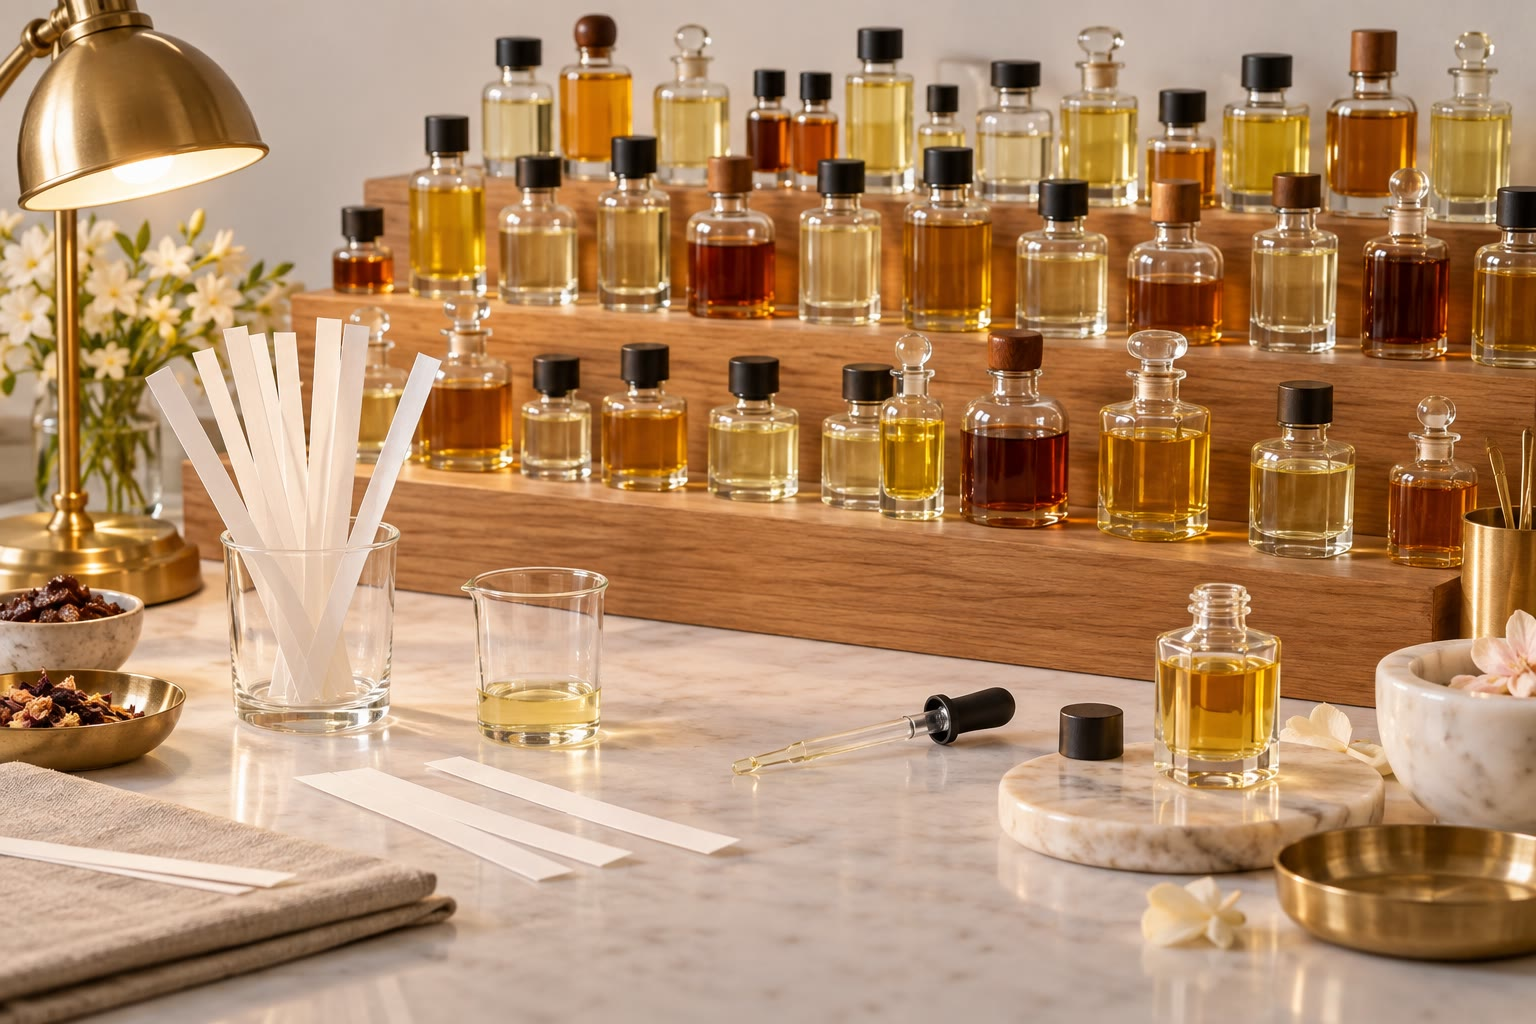
\includegraphics[width=0.48\linewidth]{images/book1/ai/g11-perfumer-lab.jpg}

{\small La paillasse d'un parfumeur~: beaucoup de flacons contiennent des
\omterm{def:g11:functional-groups:carboxylic-acid}{esters}, des \omterm{def:g11:functional-groups:alcohol}{alcools}, des \omterm{def:g11:functional-groups:carbonyl}{aldéhydes} et des \omterm{def:g11:functional-groups:carbonyl}{cétones}.}
\end{omfigure}

\begin{safety}{\ghs[0.82cm]{GHS02}\ghs[0.82cm]{GHS05}\ghs[0.82cm]{GHS07}}
% ledger: ghs:acetone, ghs:acetic-acid
La propanone est très inflammable et irritante pour les yeux~; sa
vapeur provoque la somnolence. L'acide éthanoïque pur est inflammable et
provoque de graves brûlures de la peau et des yeux~; le vinaigre en est
une solution diluée. On ne teste jamais une odeur en reniflant un
flacon~: on rabat doucement la vapeur vers le nez avec la main, et
seulement quand l'enseignant le permet.
\end{safety}

\section{Exercices}


\begin{exercise}[$\star$]\label{exo:g11:functional-groups:1}
Nommer le \omterm{def:g11:functional-groups:functional-group}{groupe caractéristique} et la famille de chaque composé~:
\ce{CH3-CH2-CH2-OH}~; \ce{CH3-CO-CH2-CH3}~; \ce{CH3-CH2-COOH}~;
\ce{CH3-COO-CH3}~; \ce{CH3-CH2-NH2}.
\end{exercise}

\begin{exercise}[$\star$]\label{exo:g11:functional-groups:2}
Nommer~: \ce{CH3-OH}~; \ce{CH3-CH2-CH2-OH}~; \ce{HCOOH}~;
\ce{CH3-CH2-CHO}~; \ce{CH3-CO-CH3}.
\end{exercise}

\begin{exercise}[$\star$]\label{exo:g11:functional-groups:3}
À quelle famille appartient chaque composé~: le butan-2-ol, le pentanal,
le propanoate de méthyle, le propanamide, le 2-bromopropane, le
but-1-ène~?
\end{exercise}

\begin{exercise}[$\star$]\label{exo:g11:functional-groups:4}
Écrire les \omterm{def:g11:organic-skeletons:formulas}{formules semi-développées} du propanal et de la propanone.
Lequel est l'\omterm{def:g11:functional-groups:carbonyl}{aldéhyde}~? Comment le reconnaît-on~?
\end{exercise}

\begin{exercise}[$\star$]\label{exo:g11:functional-groups:5}
Donner la classe du propan-1-ol, du propan-2-ol et du
2-méthylpropan-2-ol.
\end{exercise}

\begin{exercise}[$\star\star$]\label{exo:g11:functional-groups:6}
Dessiner les \omterm{def:g11:organic-skeletons:formulas}{formules topologiques} du pentan-3-ol, de l'acide
2-méthylbutanoïque, de l'hexan-2-one et de l'éthanoate de propyle.
\end{exercise}

\begin{exercise}[$\star\star$]\label{exo:g11:functional-groups:7}
Le propanal et la propanone ont la même \omterm{def:g11:organic-skeletons:formulas}{formule brute}. La donner. Sont-ils
\omterm{def:g11:organic-skeletons:isomer}{isomères}~? Ont-ils le même \omterm{def:g11:functional-groups:functional-group}{groupe caractéristique}~?
\end{exercise}

\begin{exercise}[$\star\star$]\label{exo:g11:functional-groups:8}
Écrire la \omterm{def:g11:organic-skeletons:formulas}{formule semi-développée} et le nom de l'\omterm{def:g11:functional-groups:carboxylic-acid}{ester} dont la partie
acide vient de l'acide méthanoïque \ce{HCOOH} et dont la partie \omterm{def:g11:functional-groups:alcohol}{alcool}
vient de l'éthanol~; puis ceux de l'\omterm{def:g11:functional-groups:carboxylic-acid}{ester} issu de l'acide éthanoïque et
du propan-1-ol.
\end{exercise}

\begin{exercise}[$\star\star$]\label{exo:g11:functional-groups:9}
Nommer les \omterm{def:g11:functional-groups:carboxylic-acid}{esters} \ce{CH3-COO-CH3}, \ce{CH3-CH2-COO-CH2-CH3} et
\ce{HCOO-CH3}, et donner l'acide et l'\omterm{def:g11:functional-groups:alcohol}{alcool} auxquels chacun est
apparenté.
\end{exercise}

\begin{exercise}[$\star\star$]\label{exo:g11:functional-groups:10}
Dessiner et nommer les quatre \omterm{def:g11:functional-groups:alcohol}{alcools} de formule \ce{C4H10O}, et donner
la classe de chacun.
\end{exercise}

\begin{exercise}[$\star\star$]\label{exo:g11:functional-groups:11}
À l'aide du tableau des groupes~: quelle est la famille de
\ce{CH3-CO-NH2}~? Quelle terminaison prend le nom d'un \omterm{def:g11:functional-groups:halogenoalkane}{alcène}~? Quelles
sont les familles qui ont un groupe carbonyle avec un \omterm{def:g7:atoms-and-molecules:atom}{atome}
d'oxygène ou d'azote sur le même carbone~?
\end{exercise}

\begin{exercise}[$\star\star\star$]\label{exo:g11:functional-groups:12}
Entourer et nommer les \omterm{def:g11:functional-groups:functional-group}{groupes caractéristiques} de l'aspirine et du
paracétamol. (Un \ce{-OH} lié directement à un cycle comme celui du
paracétamol s'appelle un groupe phénol~; il se comporte autrement qu'un
\omterm{def:g11:functional-groups:alcohol}{alcool}.)
\begin{center}
\setchemfig{atom sep=1.6em}
\chemfig{*6(-=-(-COOH)=(-O-[:150]C(=[:90]O)-[:210]H_3C)-=)}
\qquad
\chemfig{*6((-OH)=-=(-N(-[2]H)-[7]C(=[6]O)-[1]CH_3)-=-)}
\\[2pt] \small aspirine \hspace{4.2cm} paracétamol
\end{center}
\end{exercise}

\begin{exercise}[$\star\star\star$]\label{exo:g11:functional-groups:13}
% ledger: bp:C2H5OH, bp:CH3OCH3
L'éthanol \ce{CH3-CH2-OH} et le méthoxyméthane \ce{CH3-O-CH3} ont la
même \omterm{def:g11:organic-skeletons:formulas}{formule brute}. La donner. Le méthoxyméthane appartient à une famille
absente du tableau, les éthers-oxydes. Lequel des deux peut former des
\omterm{def:g11:polarity-and-cohesion:hydrogen-bond}{liaisons hydrogène} entre ses propres \omterm{def:g7:atoms-and-molecules:molecule}{molécules}~? Lequel bout le plus
haut (l'un bout à \qty{78}{\celsius}, l'autre à \qty{-25}{\celsius})~?
\end{exercise}

\begin{exercise}[$\star\star\star$]\label{exo:g11:functional-groups:14}
L'acide lactique, produit par les muscles fatigués, a pour formule
\chemfig{CH_3-CH(-[2]OH)-COOH}. Nommer ses deux \omterm{def:g11:functional-groups:functional-group}{groupes caractéristiques}.
Quand une \omterm{def:g7:atoms-and-molecules:molecule}{molécule} possède un groupe acide et un autre groupe, l'acide
donne la terminaison et l'autre groupe devient un préfixe
(\emph{hydroxy-} pour \ce{-OH}, \emph{amino-} pour \ce{-NH2}). Nommer
l'acide lactique, puis la glycine, \ce{H2N-CH2-COOH}.
\end{exercise}

\begin{exercise}[$\star\star\star$]\label{exo:g11:functional-groups:15}
Le vin laissé à l'\omterm{def:g4:air-a-mixture-of-gases:air}{air} se transforme en vinaigre~: l'éthanol devient de
l'acide éthanoïque, en passant par l'éthanal. Écrire les \omterm{def:g11:organic-skeletons:formulas}{formules
semi-développées} et brutes des trois composés et donner leurs familles.
Qu'est-ce qui change dans la formule à chaque étape~?
\end{exercise}

\section{Problème~: les arômes fruités}

\begin{problem}[{Problème du week-end --- une aromaticienne reconstitue
l'odeur de la banane~: quelle est la masse molaire de la molécule
clé~?}]
\label{pb:g11:functional-groups:1}
% ledger: aw:C, aw:H, aw:O
Une aromaticienne a cinq composés sur sa paillasse~:
\begin{center}
\begin{tabular}{ll}
A & \chemfig{CH_3-C(=[2]O)-O-CH_2-CH_2-CH(-[2]CH_3)-CH_3} \\[16pt]
B & \chemfig{HO-CH_2-CH_2-CH(-[2]CH_3)-CH_3} \\[10pt]
C & \ce{CH3-COOH} \\
D & \ce{CH3-CH2-CH2-CH2-CH2-CHO} \\
E & \ce{CH3-CH2-CH2-COO-CH2-CH3}
\end{tabular}
\end{center}
A sent la banane et le bonbon acidulé, B le malt, C le vinaigre, D
l'herbe coupée, E l'ananas.

\medskip
\noindent\textbf{Partie I --- Groupes et familles.}
\begin{enumerate}
  \item Nommer le \omterm{def:g11:functional-groups:functional-group}{groupe caractéristique} de chaque composé.
  \item Donner la famille de chacun.
  \item Quels composés sont des \omterm{def:g11:functional-groups:carboxylic-acid}{esters}~? Quelles odeurs ont-ils~?
  \item Quelle est la classe de l'\omterm{def:g11:functional-groups:alcohol}{alcool} B~?
  \item Donner la \omterm{def:g11:organic-skeletons:formulas}{formule brute} de D, et dessiner un \omterm{def:g11:organic-skeletons:isomer}{isomère} de D qui
        soit une \omterm{def:g11:functional-groups:carbonyl}{cétone}.
\end{enumerate}

\medskip
\noindent\textbf{Partie II --- Les noms.}
\begin{enumerate}[resume]
  \item Nommer B (chercher la plus longue chaîne qui contient le carbone
        portant le \ce{-OH}).
  \item Nommer C et D.
  \item Nommer E, et donner l'acide et l'\omterm{def:g11:functional-groups:alcohol}{alcool} auxquels il est
        apparenté.
  \item Expliquer le nom de A, éthanoate de 3-méthylbutyle~: quelle
        partie vient de l'acide, laquelle de l'\omterm{def:g11:functional-groups:alcohol}{alcool}~?
\end{enumerate}

\medskip
\noindent\textbf{Partie III --- À partir d'un acide et d'un \omterm{def:g11:functional-groups:alcohol}{alcool}.}
\begin{enumerate}[resume]
  \item À quels deux composés de la paillasse A est-il apparenté~?
  \item Donner les \omterm{def:g11:organic-skeletons:formulas}{formules brutes} de A, B et C.
  \item Un \omterm{def:g11:functional-groups:carboxylic-acid}{ester} se forme à partir de son acide et de son \omterm{def:g11:functional-groups:alcohol}{alcool} avec
        perte d'une petite \omterm{def:g7:atoms-and-molecules:molecule}{molécule}. À l'aide des formules, trouver
        laquelle.
  \item Écrire l'équation de la formation de A, en \omterm{def:g11:organic-skeletons:formulas}{formules brutes}, et
        vérifier qu'elle est ajustée.
\end{enumerate}

\medskip
\noindent\textbf{Partie IV --- Les \omterm{def:g10:the-mole:molar-mass}{masses molaires}.}
\begin{enumerate}[resume]
  \item Calculer les \omterm{def:g10:the-mole:molar-mass}{masses molaires} de B et de C.
  \item En déduire la \omterm{def:g10:the-mole:molar-mass}{masse molaire} de A à partir de l'équation de la
        question 13.
  \item Calculer directement la \omterm{def:g10:the-mole:molar-mass}{masse molaire} de A à partir de sa
        formule, et comparer.
  \item Un échantillon fruité inconnu a une \omterm{def:g10:the-mole:molar-mass}{masse molaire} proche de
        \qty{116}{g/mol}. Est-ce A ou E~?
  \item L'acide heptanoïque, \ce{CH3-(CH2)5-COOH}, sent le rance. Montrer
        que c'est un \omterm{def:g11:organic-skeletons:isomer}{isomère} de A. Une \omterm{def:g10:the-mole:molar-mass}{masse molaire} suffit-elle à
        identifier un composé~?
  \item Pourquoi les chimistes disent-ils que l'odeur tient autant au
        \omterm{def:g11:functional-groups:functional-group}{groupe caractéristique} qu'au squelette~? Utiliser A et l'acide
        heptanoïque.
  \item Donner la réponse finale~: quelle est la \omterm{def:g10:the-mole:molar-mass}{masse molaire} de
        l'\omterm{def:g11:functional-groups:carboxylic-acid}{ester} de la banane, l'éthanoate de 3-méthylbutyle~?
\end{enumerate}
\end{problem}
